\chapter{The Physics}
\section{The physical system}
The physical system to be modeled is a thin, rectangular strip of bacon which is
subjected to approx. 750 watts of microwave radiation at the frequency of 2.4
GHz. To be modeled is the heat in the strip, phase transitions and transport.

\section{Our approach}
\begin{figure}[!h]
  \begin{center}
    
\includegraphics[width=0.35\linewidth]{physicists.png}
  \end{center}
  \caption{Our initial approach to the problem. \url{xkcd.com/793}}
  \label{fig:xkcd_physics}
\end{figure}

Initially, our approach to modelling was to use a staggered approach: first solve the
heat equation for the three media meat, solid fat, and liquid fat, thus giving
the temperature at computation step $i$. Then at step $i+1$, the temperature is regarded as
known, and we solve the transport equation for liquid fat out of the bacon. Then
we know the distribution of liquid fat at step $i+2$, where we solve the heat
equations again, et cetera.

\section{The heat equations}
The differential equations governing the heat transport are all variations of the heat
equation, with various source terms, \crefrange{eq:heat1}{eq:heat3}:
\begin{align}
  \label{eq:heat1}
  (\rho c_p)_m \pd{T}{t} - \alpha_m \grad{^2 T} &= J^{MW} \quad \rm{,} \\
  \label{eq:heat2}
  \eta_s (\rho c_p)_s \pd{T}{t} - \eta_s\alpha_s \grad{^2 T} &= J^{MW} - J^{Melt}  \quad \rm{,} \\
  \label{eq:heat3}
  \eta_l (\rho c_p)_l \pd{T}{t} - \eta_s\alpha_l \grad{^2 T} - \eta_l(\rho c_p)_l(\v{v}\cdot
  \grad{})T &= J^{MW}  \quad \rm{.}
\end{align}
Here the subscript $m$ denotes meat, $s$ denotes solid fat, and $l$ denotes
liquid fat. $J^{MW}$ is the source term representing the microwave oven.
Here this is modelled as a cylindrically symmetric term,
with the radial power distribution on the form \cref{eq:effektfordeling},
\begin{equation}
  J^{MW}(r) = 0.5 + 2.55008r - 0.588013r^2 + 0.032445r^3 + 0.00124411r^4 -
  9.73516\cdot 10^{-4}r^5 \rm{,}
  \label{eq:effektfordeling}
\end{equation}
i.e. a fifth degree polynomial, interpolated from the results in
\cite{huang+zhu}. This is an effective source term, and is considered valid for
cooking times that are large compared to the rotation period of the plate inside
the microwave oven. This term may look confusing, so it has been illustrated in
\cref{fig:microwave}.\\

\begin{figure}[h!]
  \begin{center}
    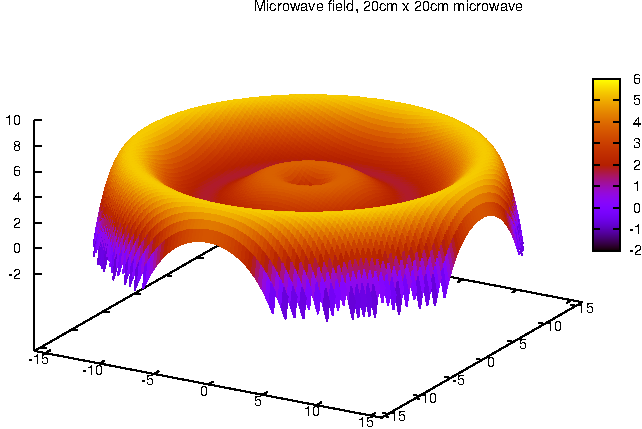
\includegraphics[width=0.7\textwidth]{microwave.pdf}
  \end{center}
  \caption{The microwave effect distribution}
  \label{fig:microwave}
\end{figure}

Furthermore, there is the term $J^{Melt}$ which represents heat loss due to
latent heat absorbed in the solid-liquid phase transition. This can be written as 
\[ \frac{L \rho}{T_2-T_1} \pd{T}{t} \rm{,} \quad T \in (T_1,T_2) \rm{,}\]
where $L$ is the latent heat of the fat, and with the fat is melting between the temperatures 
$T_1$ and $T_2$. For fat these are typically around 30-50$^\circ$C. For $T
\notin (T_1,T_2)$ 
this term is zero. It is readily seen that this is equivalent to a modification of the constant
$c_{p,l}$ in \cref{eq:heat2} when $T \in (T_1,T_2)$, thus it is not a serious
complication.\\

In the last of the heat equations, there also appears what is called a
convective derivative, on the form $(\v{v}\cdot \grad{})T$. This is a somewhat
more complicated term, and is essentially a modification due to transport of
liquid fat implying a transport of heat. But we're in luck! \\

As the bacon strip is essentially two-dimensional, transport will almost
exclusively happen in the vertical (small) direction, and the
source terms don't vary in this direction. As this term will be a transport
of heat in the vertical direction, it will not affect the heat transport in
the horisontal directions.  As we're not really
interested in the vertical temperature distribution, this means that we can
happily neglect this term. In the spirit of Richard Feynmann: ``it doesn't give
any new physics''.

\section{The transport equations}
The transport equation used in our approach is the one-dimensional Navier Stokes
equation, with the additional assumptions of an incompressible, Newtonian flow.
This is the same as ignoring phenomena where sound waves or shock waves are
important, which makes sense here. This leads to \cref{eq:navier-stokes}
\begin{equation}
  \rho \left(\pd{v}{t} + v \cdot \pd{v}{x}\right) = -\pd{p}{x} + \mu \nabla^2 v + f
 \label{eq:navier-stokes}
\end{equation}
where $f$ includes any additional forces, such as gravity. An interesting term here is $\pd{p}{x}$, where
$p$ is the pressure in the fluid. Following the work by \cite{brent}, we replace
this with a term inspired by \cref{carman-kozeny}
\begin{equation}
  \pd{p}{x} = -C\frac{ (1-\epsilon)^2}{\epsilon^3} v_a
  \label{carman-kozeny}
\end{equation}
where $\epsilon = \epsilon(z)$ is the melted fraction in the current volume element, and
$v_a$ is an apparent velocity. As the volume element melts, $\epsilon$ goes from
zero to one, and $\pd{p}{x}$ goes from a very large value to zero. This is known 
as the Carman-Kozeny equation for flow in a porous medium. It is applicable to 
materials where melting does not happen at one specific temperature, but instead 
over a range of temperatures (non-isothermal phase change). \cite{poirier} \\

This melting behavior is typical for a material with a combination of slightly different
fats, e.g. chocolate or in this case bacon. When a volume element is partially
melted, it is assumed to have a dendritic structure, and it is said to be in a
``mushy'' phase. The dendritic structure itself, and whether the flow is parallell or
orthogonal to the dendritic structure, will influence the constant C. \\

Using the procedure outlined in \cite{poirier}, the constant $C$ was measured to
be about $8 \times 10^8$. Here it has been assumed that bacon is cut orthogonal
to the dendritic fiber structure of the meat, so that the flow will be in the
parallell direction to the dendritic structure. Using this fact, along with a
measured distance of 2.5 mm between dendritic fibers in partially molten bacon, 
the procedure gives the value of the Kozeny constant previously stated.\\

Influenced by these considerations, the term $\pd{p}{x}$ in
\cref{eq:navier-stokes} was replaced by \cref{eq:pressure}
\begin{equation}
  \pd{p}{x} =  -C\frac{ (1-\epsilon)^2}{(\epsilon+d)^3} v
  \label{eq:pressure}
\end{equation}
where $d$ is a tiny constant introduced simply to avoid dividing by zero in the
numerical procedure.\\

Introducing this term has two effects. First of all, for a solid element,
$\pd{p}{x}$ becomes very large, and forces the velocity to be zero. When the
element starts melting, the flow will mimic the Carman-Kozeny flow, which is
realistic for a porous medium. Finally in the molten stage, the ordinary
pressureless Navier Stokes equations are recovered.\\

Alas, the numerical implementation of the transport equation was not completed
within the timeframe of the project. The theory is still presented here for
completeness.\\ %Paragraph check

An alternative route investigated at the last moment is to take the pressureless
Navier Stokes equation, i.e. $\pd{p}{x} = 0 \forall x,t$, and add a source term
proportional to $\pd{\epsilon}{t}$. To understand this, it helps to think of the
Navier Stokes equation as a diffusion equation in momentum, with an extra
convective derivative. With an initial condition of zero flow everywhere, and
absorbing boundary conditions, $\pd{\epsilon}{t}$ will differ from zero when
melting is happening, giving a source of momentum. This momentum is then dissipated due to
the viscosity. From experiments the fat transport seems to be isotropic, i.e.
gravity is not dominating, so the appropriate form of the whole term is
\begin{equation}
  \xi v_a \sqrt{2\pi \mu L_z} \pd{\epsilon}{t}
  \label{eq:diffusion}
\end{equation}
where $\xi$ is a random variable being either +1 or -1 with equal probability,
$v_a$ is the apparent velocity measured for liquid fat in bacon, and the scaling
factor $\sqrt{2\pi\mu L_z}$ gives the correct apparent velocity assuming
diffusion of momentum.

What has not been discussed in either of these two models is the mass
conservation equation. For a medium such as bacon, where the density may vary,
this is of the form
\begin{equation}
  \pd{\rho}{t} + \div{\rho v} = 0
  \label{massconservation}
\end{equation}
where $\rho$ is the density. This will impose a furter restriction on the
possible solutions, clearing away divergencies etc., but it also gives an
additional equation to implement
